\section{Aufbau}
\label{sec:Aufbau}
\begin{figure}
	\centering
	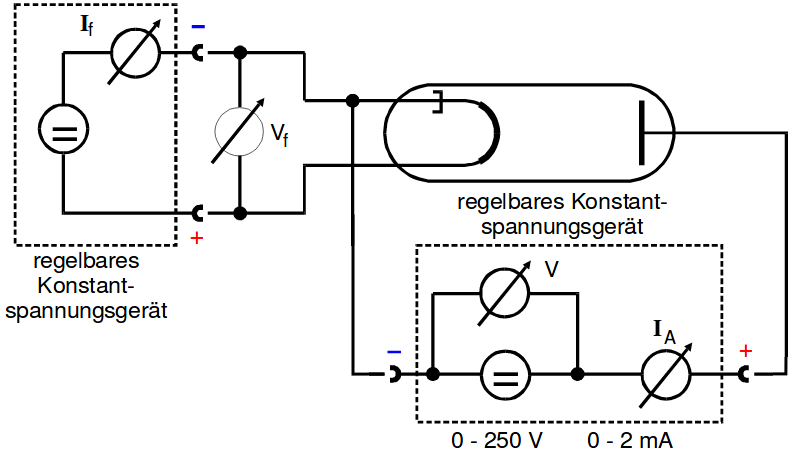
\includegraphics[width=\linewidth-100pt,height=\textheight-100pt,keepaspectratio]{content/Bilder/Schaltung1.png}
	\caption{Darstellung einer möglichen Schaltung zur Aufnahme von Kennlinien mit $V\ge0$ \cite{V504}.}
	\label{fig:Schaltung1}
\end{figure}
In Abbildung \ref{fig:Schaltung1} ist eine mögliche Schaltung zur Aufnahme von Kennlinien im Bereich $V\ge 0$ abgebildet. Ein regelbares Konstantspannungsgerät sorgt für eine regelbare konstante Heizleistung in der Hochvakuum-Diode und ein zweites regelbares Konstantspannungsgerät für eine einstellbare konstante Saugspannung. An beiden Geräten können sowohl Spannung als auch die Stromstärke abgelesen werden.
\begin{figure}
	\centering
	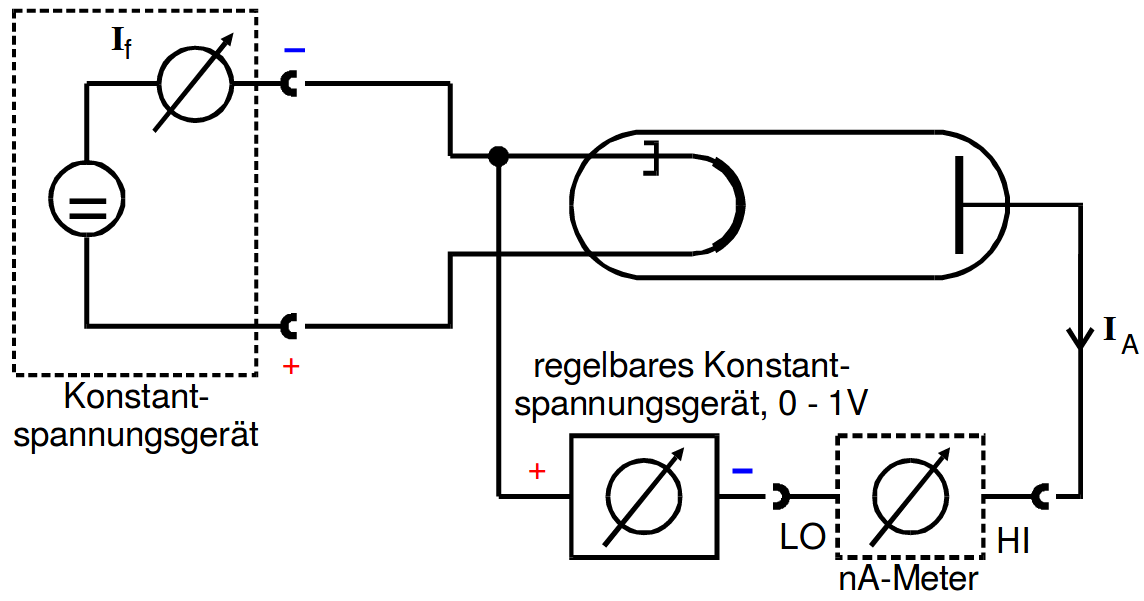
\includegraphics[width=\linewidth-100pt,height=\textheight-100pt,keepaspectratio]{content/Bilder/Schaltung2.png}
	\caption{Darstellung einer möglichen Schaltung zur Aufnahme von Kennlinien mit $V\le0$ \cite{V504}.}
	\label{fig:Schaltung2}
\end{figure}
In Abbildung \ref{fig:Schaltung2} ist eine mögliche Schaltung zur Aufnahme von einer Kennlinie im Bereich $V\le0$ abgebildet. Ein Konstantspannungsgerät sorgt für einen konstanten Heizstrom $I_\text{f}$ vom \SI{2.5}{\ampere} und ein regelbares Konstantspannungsgerät für eine regelbares annähernd kontante Gegenfeldstärke.An dem regelbarem Konstantspannungsgerät kann die Gegenspannung und am Nanoamperemeter, mit Innenwiederstand von $\SI{1}{\mega\ohm}$, die Anlaufstromstärke $I_\text{A}$ gemessen werden. Zwischen dem Nanoamperemeter und der Anode sollte aufgrund der geringen Stromstärken ein besonders kurzes Kabel verwendet weden.

